Križanje s očuvanjem konteksta \cite{crxContext} također križa dvije jedinke na mjestu točke prekida. Ovaj operator u stablo uvodi koordinate svakog pojedinog čvora. Koordinate označavaju put unutar stabla kojim se dolazi do određenog čvora. Primjer koordinata čvorova stabla dan je na slici \ref{crxContextCoordinates}. Ovakve koordinate jednostavno i jednoznačno opisuju poziciju određenog čvora unutar stabla. Primjerice, čvor s koordinatama (1,1,2) nalazi se u drugoj grani podstabla koje se nalazi u prvoj grani prvog podstabla.

\begin{figure}[H]
 	\centering
\begin{tikzpicture}
	[sibling distance=45mm, level distance=25mm,
	every node/.style={fill=blue!20,circle,draw,drop shadow, minimum height=1.5cm}]
	\node   {-}
    		child {node  {1}
    			child {node {1,1}
    				child {node{1,1,1}}
    				child {node{1,1,2}}
    			}
    		}
    		child {node {2}
        		child {node  {2,1}}
        		child {node {2,2}}
      		};
	};

\end{tikzpicture}


	\caption{Koordinate čvorova stabla}
	\label{crxContextCoordinates}
\end{figure}

\subsection{Križanje s jakim očuvanjem konteksta}
Križanje s jakim očuvanjem konteksta (\textit{eng. strong context preserved crossover - SCPC}) dopušta križanje samo onih podstabala koja imaju potpuno jednake koordinate korijena. Ovakav operator postavlja vrlo stroga ograničenja na proces križanja. U \cite{crxContext} pokazano je kako koristeći ovakav operator, postoji velika vjerojatnost da podstablo generirano na određenoj razini na određenom mjestu stabla nikada ne uspije prijeći u potomke. Ovo bi kroz generacije prouzročilo smanjivanje genetske raznolikosti, što je u potpunoj suprotnosti ulozi operatora križanja. Kako bi se ublažio ovakav utjecaj operatora križanja s jakim očuvanjem konteksta, on se nikada ne koristi samostalno, već u kombinaciji s nekim drugim operatorima križanja.

\subsection{Križanje sa slabim očuvanjem konteksta}
Kako bi se ublažila rigoroznost križanja s jakim očuvanjem konteksta, D'haeseleer \cite{crxContext} je također predložio blažu inačicu ovog križanja - križanje sa slabim očuvanjem konteksta (\textit{eng. weak context preserved crossover - WCPC}). Ova inačica kontekstnog križanja predstavlja pojednostavljenje križanja s jakim očuvanjem konteksta. Korijen podstabla prvog roditelja koje će sudjelovati u križanju odabire se između skupa čvorova za koje postoji odgovarajući čvor u drugom roditelju (jednako kao i kod križanja s jakim očuvanjem konteksta). Podstablo u drugom roditelju koje će sudjelovati u križanju odabire se tako da mu vršni čvor odgovara vršnom čvoru odabranog podstabla prvog roditelja. Drugim riječima, ako su $T1$ i $T2$ važeći odabiri podstabala za križanje s jakim očuvanjem konteksta, tada su $T1$ i $T2' \subseteq T2$ važeći odabiri podstabala za križanje sa slabim očuvanjem konteksta.

\subsection{Dosadašnji rezultati}
U \cite{crxContext} obavljena su četiri različita eksperimenta koja pokazuju učinkovitost ovih operatora križanja. U nastavku su opisani ti eksperimenti.

\subsubsection{Robot sa sposobnosti izmicanja preprekama}
Cilj ovog problema je evoluirati robota koji prelazi što veću površinu zadanog prostora, zaobilazeći pritom prepreke koje mu se nađu na putu. Pri tome, broj pokreta robota je ograničen na neki fiksni broj $n$. 

Rezultati ovog eksperimenta pokazali su kako ovo križanje nije dobro za evoluciju rješenja danog problema. Budući da evoluirani robot samo jednom izvršava svoj program predstavljen stablom, to stablo bi trebalo biti veliko i opisivati svaki korak robota. Budući da ova križanja, a pogotovo križanje s jakim očuvanjem konteksta ne potiče prijenos krajnjih podstabala rješenja, dobiven rezultat bio je i za očekivati. Na slici \ref{robot} dana je usporedba učinkovitosti uobičajenog (jednostavnog) operatora križanja, kombinacije jednostavnog i križanja s jakim očuvanjem konteksta (u omjeru 1:1) i križanja s jakim očuvanjem konteksta. Vidljivo je kako je jednostavno križanje superiorno nad kontekstnim križanjima za rješavanje ovog problema.

\begin{figure}[H]
	\centering
	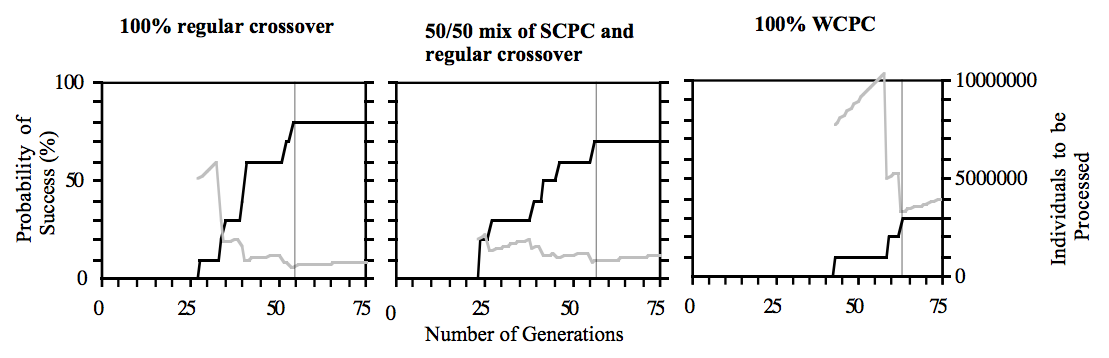
\includegraphics[scale=0.4]{./slike/robot.png}
	\caption{Učinkovitost različitih operatora križanja za problem robota sa sposobnošću izmicanja prepreka. lijevo: jednostavno križanje, sredina: kombinacija jednostavnog i križanja sa slabim očuvanjem konteksta, desno:  križanje s jakim očuvanjem konteksta (preuzeto iz \cite{crxContext})}
	\label{robot}
\end{figure}


\subsubsection{Iterirana inačica robota sa sposobnosti izmicanja preprekama}
Za razliku od prethodno opisanog problema, gdje se program predstavljen stablom izvršava samo jedan put, u ovom problemu unutar dopuštenog broja koraka dopušteno je izvoditi program po nekoliko puta. Ovakvo ponašanje u stvari je i prirodnije od jednostrukog izvršavanja stabla, i očekivano je da će u ovom slučaju kontekstni operatori djelovati efikasnije nego kod rješavanja prethodnog problema. Na slici \ref{robotIt} prikazana je usporedba učinkovitosti operatora križanja za ovaj problem. Vidljivo je kako je kombinacija jednostavnog i križanja s jakim očuvanjem konteksta (u omjeru 1:3) djelovala najbolje pri rješavanju ovog problema.

\begin{figure}[H]
	\centering
	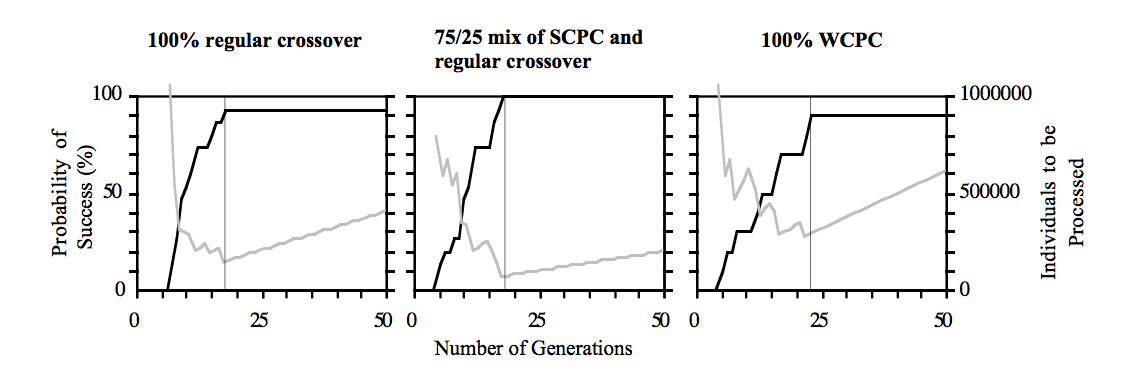
\includegraphics[scale=0.4]{./slike/robotIt.png}
	\caption{Učinkovitost različitih operatora križanja za iterativni problem robota sa sposobnošću izmicanja prepreka. lijevo: jednostavno križanje, sredina: kombinacija jednostavnog i križanja sa slabim očuvanjem konteksta, desno:  križanje s jakim očuvanjem konteksta (preuzeto iz \cite{crxContext})}
	\label{robotIt}
\end{figure}



\subsubsection{11 - multipleksor}
Cilj boolean 11 - multipleksor problema je pronaći logičku funkciju koja za 3 predana adresna bita daje podatak veličine 8 bita. U ovom problemu, kombinacija jednostavnog i križanja s jakim očuvanjem konteksta (u omjeru 1:1) pokazala se daleko boljim odabirom za operator križanja nego jednostavno križanje. Križanje sa slabim očuvanjem konteksta se i u ovom eksperimentu pokazalo prilično inferiorno ostalim dvama operatorima. Na slici \ref{mux} prikazana je usporedba učinkovitosti različitih operatora križanja na ovaj problem.

\begin{figure}[H]
	\centering
	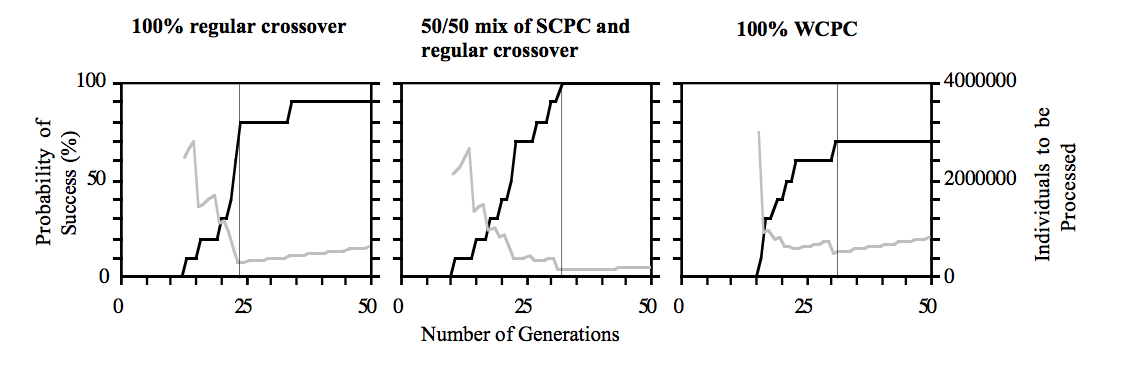
\includegraphics[scale=0.4]{./slike/mux.png}
	\caption{Učinkovitost različitih operatora križanja za problem boolean 11 - multipleksora. lijevo: jednostavno križanje, sredina: kombinacija jednostavnog i križanja sa slabim očuvanjem konteksta, desno:  križanje s jakim očuvanjem konteksta (preuzeto iz \cite{crxContext})}
	\label{mux}
\end{figure}



\subsubsection{Centralno sakupljalište hrane}
Efikasno rješenje ovog problema je evoluirani program koji, kada je pokrenut nad svakim umjetnim mravom kolonije, prouzrokuje transport sve hrane s danog područja na jedno, centralno mjesto. Dobro rješenje ovog problema mora uključivati i interakciju i kooperaciju između mrava. Radi toga, evoluirani program najčešće su kratki, sadržavajući samo nekoliko koraka u svakoj iteraciji izvođenja. Ovo upućuje na činjenicu da bi kontekstno križanje moglo biti vrlo korisno za evoluciju takvog, efikasnog rješenja. Na slici \ref{ants}, jednako kao i za prethodne eksperimente, prikazana je usporedba učinkovitosti različitih operatora križanja na ovaj problem.

\begin{figure}[H]
	\centering
	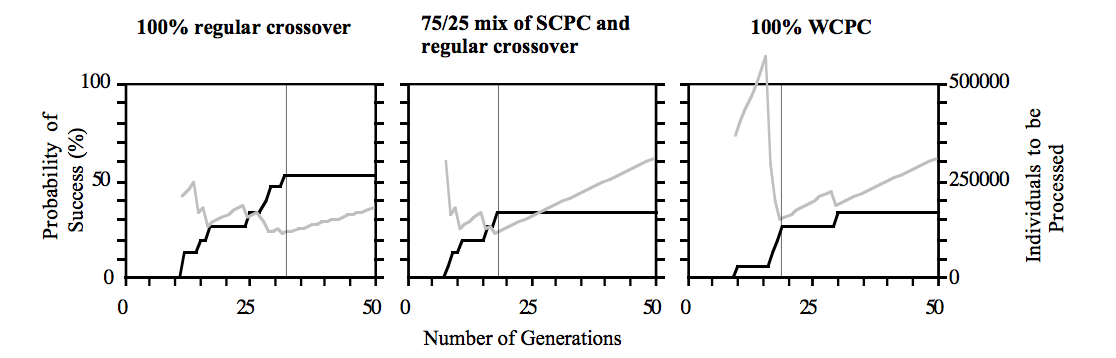
\includegraphics[scale=0.4]{./slike/ants.png}
	\caption{Učinkovitost različitih operatora križanja za problem centralnog sakupljališta hrane. lijevo: jednostavno križanje, sredina: kombinacija jednostavnog i križanja sa slabim očuvanjem konteksta, desno:  križanje s jakim očuvanjem konteksta (preuzeto iz \cite{crxContext})}
	\label{ants}
\end{figure}



Ova istraživanja pokazala su kako križanje s očuvanjem konteksta nije učinkovito kada je upotrebljeno samo, već je efikasnije u kombinaciji s nekim drugim operatorom. Kombinacija jednostavnog križanja i križanja s jakim očuvanjem konteksta pokazala se kao vrlo učinkovit operator za iterirane programe koji predstavljaju neovisnu jedinku i za pronalazak logičkih funkcija.

